\documentclass[11pt,a4paper]{article}
\usepackage[utf8]{inputenc}
\usepackage[T1]{fontenc}
\usepackage{lmodern}
\usepackage[margin=2.1cm]{geometry}
\usepackage{amsmath,amssymb,amsthm,mathtools}
\usepackage{booktabs,tabularx,array}
\usepackage{graphicx}
\usepackage{xcolor}
\usepackage{enumitem}
\usepackage{microtype}
\usepackage[colorlinks=true,linkcolor=blue!55!black,citecolor=blue!55!black,urlcolor=blue!55!black]{hyperref}

\setlength{\emergencystretch}{3em}
\newtheorem{theorem}{Theorem}[section]
\newtheorem{proposition}[theorem]{Proposition}
\newtheorem{corollary}[theorem]{Corollary}
\newtheorem{remark}[theorem]{Remark}

\title{\textbf{Scale-Invariant Simplicial $R^2$ Inflation, Multi-Sector $CP$ Structure,\\
and Zero-Parameter Non-Thermal Scalaron Leptogenesis\\
from a Tetrahedral $\mathrm{Spin}(10)$ Threshold}\\[0.35em]
\large First-Principles Coleman--Weinberg Supertrace, $\mathrm{SO}(2,\mathbb{C})$ Casas--Ibarra Geometry, and Four-Experiment Falsification}

\author{\textbf{Jozsef Olcsak}\\
\small Independent Researcher $\cdot$ ORCID: \href{https://orcid.org/0009-0003-7311-6522}{0009-0003-7311-6522}\\
\small Email: \href{mailto:jolcsak@gmail.com}{jolcsak@gmail.com} $\cdot$ Code \& Data Archive: \href{https://doi.org/10.5281/zenodo.24379738}{doi:10.5281/zenodo.24379738}}
\date{19 November 2026}

\begin{document}
\maketitle

\begin{abstract}
\noindent Joint models of Starobinsky $R^2$ inflation, Type-I seesaw neutrino masses, and post-inflationary leptogenesis typically introduce five to seven independent parameters ($M_{\mathrm{inf}}, M_1, M_2, \operatorname{Re}z, \operatorname{Im}z, \xi_H, \bar{\theta}_{\mathrm{QCD}}$). Here we investigate whether the entire ultraviolet-to-electroweak sequence is fixed without added free parameters ($k_{\mathrm{added}} = 0$) once the four-vertex tetrahedral simplicial-Clifford invariant $u = \sqrt{N-1}/N! = \sqrt{3}/24$ ($N=4$) and its chiral $\mathrm{Spin}(10)$ seesaw threshold $M_R = M_*/(256\pi^2) = 5.565\times 10^{14}\;\mathrm{GeV}$ ($M_* = M_{\mathrm{Pl}}/\sqrt{3}$) are specified. First, we prove two sharp no-go theorems: (i) low-energy unit-timelike vector-director gravity rescales only the cosmological Newton constant on spatially flat FLRW backgrounds without generating slow-roll inflation; and (ii) minimally coupled 1-loop Schwinger--DeWitt $a_2(x)$ matter heat kernels contribute zero local $R^2$ for massless spin-$1/2$ and spin-$1$ fields and $\Delta\beta_{R^2} \le 0.145$ for $N_0 \le 210$ real scalars, falling short of the Starobinsky stiffness $\beta_{R^2}^{\mathrm{Star}} = 2^{22}\cdot 3\,\pi^6 / 25 = 4.839\times 10^8$ by a factor $>3.34\times 10^9$. Second, we prove via computer algebra (\texttt{SymPy}) that eliminating the traceless-Hessian auxiliary plaquette constraint $\mathcal{L}_{\mathrm{HS}} = \frac{1}{2}M_{\mathrm{Pl}}^2 R + \frac{1}{\sqrt{2}}M_*\sigma R - \frac{1}{2}m_\sigma^2\sigma^2$ yields $\frac{1}{2}M_{\mathrm{Pl}}^2(R + R^2/6m_\sigma^2)$ identically, while under a classical scale-invariant ultraviolet boundary condition (\texttt{BC-UV-CW}) the 1-loop Coleman--Weinberg supertrace between $d_A(N) = (N-1)^2 - 1$ real bosonic and $2d_S(N) = 2(N-1)$ real Majorana threshold degrees of freedom at $M_R$ is tachyonic ($-1$) at $N=3$ but uniquely positive ($8 - 6 = +2$) at $N=4$. The irrational $\sqrt{3}$ cancels identically in $M_{\mathrm{inf}}/M_{\mathrm{Pl}} = \frac{N+1}{32\pi^3 N! N^2}\big|_{N=4} = \frac{5}{12{,}288\pi^3}$, fixing $M_{\mathrm{inf}} = \frac{5u}{2\pi}M_R = 3.196\times 10^{13}\;\mathrm{GeV}$. Exact Klein--Gordon integration with self-consistent Liddle--Leach reheating ($N_* = 51.41$, $T_{\mathrm{rh}} = 5.13\times 10^9\;\mathrm{GeV}$ at $\xi_H = 0$) yields next-to-leading-order CMB observables $A_s = 2.101\times 10^{-9}$ ($+0.04\sigma$ vs.\ \texttt{Planck 2018}), $n_s = 0.9620$ ($-0.69\sigma$), and $r = 0.00426$. Third, while inflation dilutes any pre-inflationary bounce asymmetry by $e^{-3N_*}\simeq 10^{-67}$, gravitational scalaron decay opens kinematically exclusively into the lightest rank-2 seesaw state $\phi \to N_1 N_1$ ($\mathrm{BR} = 1.28\%$, $M_1 = 5.696\times 10^{12}\;\mathrm{GeV} < M_{\mathrm{inf}}/2 < M_2$). Cartan polar decomposition of the complex orthogonal Casas--Ibarra matrix $\mathbf{R}(\theta_\tau + i u) = \mathbf{O}(\theta_\tau)\mathbf{H}(u) \in \mathrm{SO}(2,\mathbb{C})$ unites $\sin\theta_\tau = 3/(8\sqrt{2})$ with the tangential chiral Wick boost $u = \sqrt{3}/24$ ($|\varepsilon_1| = 8.470\times 10^{-5}$), yielding via stiff 4-species Radau Boltzmann integration $\eta_B = 6.104\times 10^{-10}$ ($-0.41\sigma$ vs.\ \texttt{Planck 2018} for $c_{\mathrm{sph}} = 28/79$; $5.585\times 10^{-10}$ for $12/37$ crossover), alongside tree-level $\bar{\theta}_{\mathrm{QCD}} = 0$ without axions. Joint falsification criteria are locked for \texttt{LiteBIRD}/\texttt{CMB-S4}, \texttt{DUNE}/\texttt{Hyper-Kamiokande}, \texttt{LEGEND-1000}, and \texttt{n2EDM}.
\end{abstract}

\tableofcontents
\vspace{0.4em}
\hrule
\vspace{0.8em}

% =============================================================================
\section{Introduction}
\label{sec:intro}
% =============================================================================

Two of the best-motivated extensions of the Standard Model (SM) and General Relativity (GR) are Starobinsky quadratic curvature inflation \cite{Starobinsky1980,MukhanovChibisov1981} and Type-I seesaw leptogenesis \cite{FukugitaYanagida1986,BuchmullerDiBariPlumacher2005}. Starobinsky's $\mathcal{L} = \frac{1}{2}M_{\mathrm{Pl}}^2(R + R^2/6M_{\mathrm{inf}}^2)$ action requires no fundamental slow-roll potential parameters beyond the scalaron mass $M_{\mathrm{inf}} \simeq 3\times 10^{13}\;\mathrm{GeV}$, sits near the center of the \texttt{Planck 2018} + \texttt{BICEP/Keck} $(n_s, r)$ confidence contours \cite{Planck2018Inflation,BICEPKeck2021}, and naturally reheats the Universe through universal conformal trace couplings, including non-thermal right-handed Majorana neutrino pair production $\phi \to N_1 N_1$ when $M_1 < M_{\mathrm{inf}}/2$ \cite{GorbunovPanin2011,GorbunovTokareva2013}.

Despite this structural economy, standard treatments of Starobinsky inflation and seesaw leptogenesis leave a set of disconnected free scales and phases:
\begin{enumerate}[label=(\arabic*),leftmargin=1.8em,itemsep=2pt]
\item \emph{The scalaron stiffness puzzle:} Why is the dimensionless $R^2$ coupling $\beta_{R^2} = M_{\mathrm{Pl}}^2 / (12 M_{\mathrm{inf}}^2) \simeq 4.8\times 10^8$ nearly nine orders of magnitude larger than naive 1-loop trace anomalies, corresponding to $M_{\mathrm{inf}}/M_{\mathrm{Pl}} \simeq 1.31\times 10^{-5}$?
\item \emph{The kinematic gate puzzle:} Why does the lightest heavy Majorana state $M_1$ lie just below the decay threshold $M_{\mathrm{inf}}/2 \simeq 1.6\times 10^{13}\;\mathrm{GeV}$ while heavier states $M_{2,3}$ lie above it, preventing strong thermal washout during reheating?
\item \emph{The multi-sector $CP$ puzzle:} Why is $CP$ symmetry strongly violated in weak/leptonic interactions ($\delta_{\mathrm{CP}}^{\mathrm{PMNS}} \sim -\pi/2$ and high-scale Casas--Ibarra rapidity $\operatorname{Im}z \neq 0$) yet conserved to better than $10^{-10}$ in quantum chromodynamics ($\bar{\theta}_{\mathrm{QCD}} \simeq 0$) without observed axions \cite{Abel2020nEDM}?
\end{enumerate}

In the simplicial-Clifford unification program developed in companion studies \cite{Olcsak2026Zenodo}, low-energy gravitational and particle-physics constants emerge from the four-vertex complete graph $K_4$ ($N = 4$) equipped with unit-trace Clifford projectors in $\mathrm{Cl}(3,1)$ and chiral $\mathrm{Spin}(10)$ spinor representations. That discrete geometry locks a single fundamental spectral quantum:
\begin{equation}
u := \frac{\sqrt{N - 1}}{N!}\Bigg|_{N=4} = \frac{\sqrt{3}}{24} = 0.0721687836,
\label{eq:u-generator}
\end{equation}
from which the projector trace norm $r_{\mathrm{seed}} = 1/N = 1/4$, the positive longitudinal Hodge-defect eigenvalue $\alpha_{\mathrm{trace}} = (N+1)u = \frac{5\sqrt{3}}{24} = 0.3608439$, the tangential kinetic stiffness $K_T = 1 + u$, the simplicial plaquette scale $\ell_* = \sqrt{N!\,\pi}\,\ell_P = \sqrt{24\pi}\,\ell_P$ (hence $M_* = E_{\mathrm{Pl}}/\sqrt{24\pi} \equiv M_{\mathrm{Pl}}/\sqrt{3} = 1.406035\times 10^{18}\;\mathrm{GeV}$, where $M_{\mathrm{Pl}} = E_{\mathrm{Pl}}/\sqrt{8\pi} = 2.435323\times 10^{18}\;\mathrm{GeV}$), and the 1-loop Passarino--Veltman seesaw threshold $M_R = \frac{r_{\mathrm{seed}}^2}{16\pi^2}M_* = 5.56489\times 10^{14}\;\mathrm{GeV}$ were previously fixed without continuous free parameters ($k = 0$).

In the present paper we test whether these already-frozen constants close primordial inflation, reheating, multi-sector $CP/CPT$ symmetry, and the cosmic baryon asymmetry $\eta_B$ \emph{without introducing any new adjustable parameter} ($k_{\mathrm{added}} = 0$). Throughout, we separate unconditional mathematical no-go theorems from conditional quantum-field-theoretic derivations whose ultraviolet boundary assumptions (\texttt{BC-UV-CW}) are stated explicitly.

% =============================================================================
\section{Simplicial Scale Hierarchy and Exact Ultraviolet/Infrared No-Go Theorems}
\label{sec:nogo}
% =============================================================================

\subsection{Frozen Seesaw Mass Spectrum from $N = 4$}

On the three-dimensional zero-sum vertex subspace $V_3 = P_\perp(\mathbb{R}^4)$ orthogonal to the temporal clock vertex $v_0$ ($d_S = \dim V_3 = N - 1 = 3$), the adjoint orientation algebra has dimension $d_A = \dim\mathfrak{su}(V_3) = (N-1)^2 - 1 = 8$, and three chiral $\mathbf{16}_L$ generations of $\mathrm{Spin}(10) \subset \mathrm{Cl}(10)$ span $d_{\mathrm{Weyl}} = 16\,d_S = 2\,d_S d_A = 48$ two-component Weyl spinors. Operational reflection positivity excludes the unoriented null mode ($\mathcal{D}_{\mathrm{OS}}^{\mathrm{op}}(0) = 0 \implies m_1 = 0$), reducing the active Type-I seesaw sector to rank $2$ with heavy Majorana eigenstates:
\begin{align}
M_2 &\equiv M_{R,3} = \frac{M_R}{3} = \frac{r_{\mathrm{seed}}^2}{48\pi^2}\,M_* = 1.85496\times 10^{14}\;\mathrm{GeV}, \label{eq:M2}\\
\eta_{\mathrm{seesaw}} &= \frac{(192u - 9)^2}{768} = \frac{(8\sqrt{3} - 9)^2}{768} = 0.0307092236, \label{eq:eta-seesaw}\\
M_1 &= \eta_{\mathrm{seesaw}}\,M_2 = 5.69644\times 10^{12}\;\mathrm{GeV}, \label{eq:M1}
\end{align}
and normal-ordered light neutrino eigenvalues $(m_1, m_2, m_3) = (0,\;8.83118,\;50.36070)\;\mathrm{meV}$ ($\Delta m_{31}^2 = 2.5362\times 10^{-3}\;\mathrm{eV}^2$, $+0.93\sigma$ vs.\ \texttt{NuFIT 6.0} \cite{Esteban2024NuFIT6}; $\sum m_\nu = 59.19\;\mathrm{meV}$).

\subsection{Infrared Vector-Director FLRW No-Go and Minimal 1-Loop Heat-Kernel No-Go}

Before constructing the ultraviolet completion, we establish two exact no-go results ruling out naive inflationary mechanisms.

\begin{proposition}[Homogeneous FLRW Vector-Director Inflation No-Go]
\label{prop:ir-nogo}
Consider the low-energy covariant unit-timelike vector-director action on a spatially flat FLRW metric $\mathrm{d}s^2 = -\mathrm{d}t^2 + a(t)^2\mathrm{d}\mathbf{x}^2$,
\begin{equation}
\mathcal{L}_{\mathrm{IR}} = \frac{M_{\mathrm{Pl}}^2}{2}R - \frac{K_B}{4}F_{\mu\nu}F^{\mu\nu} - \frac{M_{\mathrm{Pl}}^2 c_2^{\mathrm{reg}}}{2}(\nabla_\mu A^\mu)^2 + \lambda_{\mathrm{ae}}(A_\mu A^\mu + 1) + \mathcal{L}_{\mathrm{QUMOND}}(\phi_N, h^{\mu\nu}\partial_\mu\phi_N),
\end{equation}
where $F_{\mu\nu} = \nabla_\mu A_\nu - \nabla_\nu A_\mu$ and $h^{\mu\nu} = g^{\mu\nu} + A^\mu A^\nu$. On any homogeneous isotropic background, $A_\mu = (-1, \mathbf{0})$, $F_{\mu\nu} \equiv 0$, $h^{\mu\nu}\partial_\mu\phi_N \equiv 0$, and $\nabla_\mu A^\mu = 3H(t)$. Variation yields the modified Friedmann equation
\begin{equation}
3 M_{\mathrm{Pl}}^2\left(1 + \frac{3}{2}c_2^{\mathrm{reg}}\right) H^2 = \rho_{\mathrm{matter}} \iff G_{\mathrm{cosmo}} = \frac{G_N}{1 + \frac{3}{2}c_2^{\mathrm{reg}}}.
\label{eq:g-cosmo}
\end{equation}
Consequently, $\mathcal{L}_{\mathrm{IR}}$ introduces no dynamical scalar inflaton on FLRW and cannot generate a slow-roll de Sitter plateau, while $c_2^{\mathrm{reg}} \le 10^{-4}$ guarantees $|\Delta G_{\mathrm{cosmo}}/G_N| \le 1.5\times 10^{-4} \ll 10^{-2}$ throughout Big Bang Nucleosynthesis (BBN).
\end{proposition}

\begin{theorem}[Minimal 1-Loop Schwinger--DeWitt $a_2(x)$ Curvature No-Go]
\label{thm:a2-nogo}
In $D = 4$ curved spacetime, consider $N_0$ real scalars with curvature coupling $-\frac{1}{2}\xi R\phi^2$, $N_{1/2}$ massless two-component Weyl fermions, and $N_1$ Yang--Mills gauge vectors running between $\mu_{\mathrm{UV}} = M_*$ and $\mu_{\mathrm{IR}} = M_R$. In the 1-loop Schwinger--DeWitt effective action $\Delta\mathcal{L}_{\mathrm{1\text{-}loop}} = (16\pi^2)^{-1} a_2(x)\ln(M_*^2/M_R^2)$ \cite{BirrellDavies1982}:
\begin{enumerate}[label=(\alph*),leftmargin=1.8em,itemsep=2pt]
\item Massless spin-$1/2$ Weyl spinors and spin-$1$ gauge bosons are classically Weyl-invariant in $D = 4$; their $a_2(x)$ coefficients contain only $C_{\mu\nu\rho\sigma}C^{\mu\nu\rho\sigma}$, the Gauss--Bonnet density $E_4$, and $\Box R$, contributing \textbf{identically zero} to the local $R^2$ coupling: $\Delta\beta_{R^2}^{(1/2)} = \Delta\beta_{R^2}^{(1)} \equiv 0$.
\item Minimally coupled real scalars ($\xi = 0$) contribute
\begin{equation}
\Delta\beta_{R^2}^{(0)}(\xi = 0) = \frac{N_0}{64\pi^2}\left(0 - \frac{1}{6}\right)^2\ln\frac{M_*^2}{M_R^2} = \frac{N_0}{2{,}304\,\pi^2}\ln(256\pi^2)^2 = 6.891\times 10^{-4}\,N_0.
\end{equation}
Even for $N_0 = 15$ ($\Delta\beta_{R^2} = 0.0103$) or an entire $\mathrm{Spin}(10)$ scalar sector $N_0 = 210$ ($\Delta\beta_{R^2} = 0.1447$), minimal 1-loop generation falls short of the observed Starobinsky stiffness $\beta_{R^2}^{\mathrm{Star}} \simeq 4.839\times 10^8$ by a factor exceeding $\mathbf{3.34\times 10^9}$.
\end{enumerate}
\end{theorem}

% =============================================================================
\section{First-Principles Starobinsky--$K_4$ Scalaron Mass and NLO CMB Spectrum}
\label{sec:inflation}
% =============================================================================

Theorem~\ref{thm:a2-nogo} proves that a realistic $R^2$ plateau requires a non-perturbative or scale-invariant auxiliary/portal mechanism rather than minimal matter loops on bare Einstein--Hilbert gravity. On the $K_4$ complex, the internal 15-channel Hodge-defect operator $T_{\mathrm{def}}^{(15)}$ is identically traceless ($\operatorname{Tr}T_{\mathrm{def}}^{(15)} = 0$), while on the $4\times 4$ body-clock reduction space its block matrix takes the exact form
\begin{equation}
T_{\mathrm{def}} = u \begin{pmatrix} 0 & \sqrt{15} & 0 & 0 \\ \sqrt{15} & 2 & 0 & 0 \\ 0 & 0 & -1 & 0 \\ 0 & 0 & 0 & -1 \end{pmatrix}, \qquad \operatorname{spec}(T_{\mathrm{def}}) = \bigl\{+5u,\;-3u,\;-u,\;-u\bigr\},
\label{eq:tdef-matrix}
\end{equation}
exhibiting a unique positive longitudinal dilatation channel $\lambda_+ = +5u = \alpha_{\mathrm{trace}}$ and a degenerate two-dimensional transverse block $T_{\mathrm{def}}|_{(3,4)} = -u\,\mathbf{I}_2$. Because $\operatorname{Tr}T_{\mathrm{def}}^{(15)} = 0$, the pure scalar trace constraint $\sigma$ carries zero bare tree-level kinetic weight ($Z_\sigma^{\mathrm{bare}} = 0$) and enters the ultraviolet gravitational action as a Hubbard--Stratonovich auxiliary multiplier coupled linearly at the plaquette scale $M_*$.

\begin{theorem}[Plaquette Auxiliary Portal, $\sqrt{3}$-Cancellation, and $N = 4$ Coleman--Weinberg Supertrace]
\label{thm:scalaron-derivation}
Consider the plaquette auxiliary curvature-portal Lagrangian in $D = 4$ Jordan frame:
\begin{equation}
\mathcal{L}_{\mathrm{HS}}(\sigma, g) = \frac{M_{\mathrm{Pl}}^2}{2}\,R + \frac{M_*}{\sqrt{2}}\,\sigma\,R - V_{\mathrm{eff}}(\sigma), \qquad M_* = \sqrt{\frac{8}{N!}}\,M_{\mathrm{Pl}}\Bigg|_{N=4} = \frac{M_{\mathrm{Pl}}}{\sqrt{3}}.
\label{eq:hs-portal}
\end{equation}
Assume the ultraviolet boundary condition \texttt{BC-UV-CW}: (i) classical ultraviolet scale invariance sets the bare tree-level mass to zero, $m_{\sigma,0}^2(M_*) = 0$; (ii) $\sigma$ couples along the unique positive longitudinal eigenchannel $\lambda_+ = \alpha_{\mathrm{trace}} = (N+1)u$ to a degenerate threshold multiplet at $M_R$ comprising $d_A(N) = (N-1)^2 - 1$ real bosonic adjoint scalars and $d_S(N) = N - 1$ Majorana right-handed neutrinos ($2d_S(N)$ real fermionic degrees of freedom); and (iii) quadratic auxiliary dominance $V_{\mathrm{eff}}(\sigma) \simeq \frac{1}{2}m_\sigma^2\sigma^2$ holds across the inflationary curvature regime $\sqrt{R_J} < M_R$. Then (\texttt{SymPy}-verified):
\begin{enumerate}[label=(\alph*),leftmargin=1.8em,itemsep=3pt]
\item \textbf{Unique $N = 4$ Non-Tachyonic Supertrace:} The net 1-loop Coleman--Weinberg supertrace multiplicity \cite{ColemanWeinberg1973,GildenerWeinberg1976} is
\begin{equation}
n_{\mathrm{eff}}^{\mathrm{STr}}(N) := d_A(N) - 2\,d_S(N) = \bigl[(N-1)^2 - 1\bigr] - 2(N-1) = \begin{cases} -1 < 0 & (N = 3,\;\text{tachyonic instability}), \\ \mathbf{+2 > 0} & (\mathbf{N = 4,\;\text{stable minimum}}). \end{cases}
\label{eq:supertrace}
\end{equation}
At $N = 4$ ($d_A = 8$, $2d_S = 6$), the tadpole-free 1-loop Coleman--Weinberg potential renormalized at $\mu = M_R$,
\begin{equation}
V_{\mathrm{CW}}(\sigma) = \frac{n_{\mathrm{eff}}^{\mathrm{STr}}}{64\pi^2}\left[\bigl(M_R + \alpha_{\mathrm{trace}}\sigma\bigr)^4\left(\ln\frac{(M_R + \alpha_{\mathrm{trace}}\sigma)^2}{M_R^2} - \frac{1}{2}\right) + \frac{1}{2}M_R^4\right],
\end{equation}
satisfies $V_{\mathrm{CW}}(0) = 0$, $V_{\mathrm{CW}}'(0) = 0$, and exact curvature
\begin{equation}
m_\sigma^2 := V_{\mathrm{CW}}''(0) = \frac{2\,\alpha_{\mathrm{trace}}^2}{8\pi^2}\,M_R^2 = \frac{\alpha_{\mathrm{trace}}^2}{4\pi^2}\,M_R^2 = \frac{25}{768\pi^2}\,M_R^2.
\label{eq:msigma-cw}
\end{equation}
\item \textbf{Exact Emergence of Starobinsky's $1/6$ Factor and $\sqrt{3}$ Cancellation:} Eliminating $\sigma = \frac{M_*}{\sqrt{2}\,m_\sigma^2}R$ from Eq.~\eqref{eq:hs-portal} gives, by virtue of $M_*^2 / M_{\mathrm{Pl}}^2 = 1/3$,
\begin{equation}
\mathcal{L}_{\mathrm{eff}}(g) = \frac{M_{\mathrm{Pl}}^2}{2}\,R + \frac{M_*^2}{4\,m_\sigma^2}\,R^2 \equiv \frac{M_{\mathrm{Pl}}^2}{2}\!\left(R + \frac{R^2}{6\,m_\sigma^2}\right) \implies M_{\mathrm{inf}} \equiv m_\sigma = \frac{\alpha_{\mathrm{trace}}}{2\pi}\,M_R.
\label{eq:starobinsky-emergence}
\end{equation}
In the dimensionless ratio $M_{\mathrm{inf}}/M_{\mathrm{Pl}}$, the irrational factor $\sqrt{N-1} = \sqrt{3}$ cancels identically between $\alpha_{\mathrm{trace}} = \frac{5\sqrt{3}}{24}$ and $M_*/M_{\mathrm{Pl}} = \frac{1}{\sqrt{3}}$:
\begin{equation}
\boxed{\frac{M_{\mathrm{inf}}}{M_{\mathrm{Pl}}} = \frac{N + 1}{32\,\pi^3\,N!\,N^2}\Bigg|_{N=4} = \frac{5}{12{,}288\,\pi^3} = 1.3123183\times 10^{-5}, \qquad M_{\mathrm{inf}} = 3.19592\times 10^{13}\;\mathrm{GeV},}
\label{eq:minf-exact}
\end{equation}
corresponding to $\beta_{R^2}^{\mathrm{Star}} = \frac{M_{\mathrm{Pl}}^2}{12 M_{\mathrm{inf}}^2} = \frac{2^{22}\cdot 3\,\pi^6}{25} = 4.83883\times 10^8$.
\item \textbf{Dual Dynamical Portal Realization and Perturbative Unitarity:} A dynamical radial scalar $\Phi$ with non-minimal curvature coupling $\frac{1}{2}\xi_\Phi \Phi^2 R - \frac{1}{4}\lambda_\Phi(\Phi^2 - M_R^2)^2$ at $\xi_\Phi = M_*/M_R = 256\pi^2 = 2{,}526.6$ and 1-loop quartic $\lambda_\Phi = (\alpha_{\mathrm{trace}}/2\pi)^2 = 3.298\times 10^{-3}$ \cite{BezrukovShaposhnikov2008} reproduces the identical plateau ratio $\xi_\Phi/\sqrt{\lambda_\Phi} = M_*/M_{\mathrm{inf}} = 43{,}995$ ($r = 0.0042603$) while maintaining vacuum perturbative unitarity up to $\Lambda_{\mathrm{unit}}^{\mathrm{vac}} = M_{\mathrm{Pl}}/\xi_\Phi = \sqrt{3}M_R = 9.64\times 10^{14}\;\mathrm{GeV} = 61.2\,H_*$.
\end{enumerate}
\end{theorem}

\subsection{Exact Klein--Gordon Dynamics, Liddle--Leach Reheating, and NLO CMB Spectrum}

Weyl-transforming Eq.~\eqref{eq:starobinsky-emergence} to the Einstein frame via $g_{\mu\nu}^E = \Omega^2 g_{\mu\nu}$ with $\Omega^2 = 1 + R_J/(3M_{\mathrm{inf}}^2) = e^{\sqrt{2/3}\,\phi/M_{\mathrm{Pl}}}$ yields the canonical potential
\begin{equation}
V(\phi) = \frac{3}{4}\,M_{\mathrm{Pl}}^2\,M_{\mathrm{inf}}^2\left(1 - e^{-\sqrt{2/3}\,\phi/M_{\mathrm{Pl}}}\right)^2.
\label{eq:v-star}
\end{equation}
For minimally coupled SM Higgs ($\xi_H = 0$), the scalaron decays universally through its trace coupling into the 4 real Higgs components, 1-loop $\mathrm{SU}(3)_c$ gluons ($b_3 = -7$ above $M_{\mathrm{EW}}$; or $19/2$ anomalous trace coefficient), and kinematically accessible Majorana pairs $N_1 N_1$ ($2M_1 = 1.139\times 10^{13}\;\mathrm{GeV} < M_{\mathrm{inf}}$, whereas $2M_2 = 3.71\times 10^{14}\;\mathrm{GeV} \gg M_{\mathrm{inf}}$ is strictly forbidden) \cite{GorbunovPanin2011}:
\begin{align}
\Gamma(\phi \to HH) &= \frac{M_{\mathrm{inf}}^3}{48\pi M_{\mathrm{Pl}}^2} = 36.498\;\mathrm{GeV}, \qquad
\Gamma(\phi \to N_1 N_1) = \frac{M_{\mathrm{inf}} M_1^2}{96\pi M_{\mathrm{Pl}}^2}\left(1 - \frac{4M_1^2}{M_{\mathrm{inf}}^2}\right)^{3/2} = 0.4729\;\mathrm{GeV}, \label{eq:scalaron-widths}
\end{align}
giving $\Gamma_\phi^{\mathrm{tot}} = 37.035\;\mathrm{GeV}$, branching ratio $\mathrm{BR}(\phi \to N_1 N_1) = \mathbf{1.2768\%}$, and reheating temperature $T_{\mathrm{rh}} = (90 \Gamma_\phi^2 M_{\mathrm{Pl}}^2 / \pi^2 g_*)^{1/4} = 5.134\times 10^9\;\mathrm{GeV}$ ($g_* = 106.75$).

Integrating the exact nonlinear Klein--Gordon equation $\frac{\mathrm{d}^2 x}{\mathrm{d}N^2} + (3 - \epsilon_1)\bigl(\frac{\mathrm{d}x}{\mathrm{d}N} + \frac{\mathrm{d}\ln V}{\mathrm{d}x}\bigr) = 0$ ($x := \phi/M_{\mathrm{Pl}}$, $\epsilon_1 = \frac{1}{2}x'^2$) and solving the Liddle--Leach pivot matching condition \cite{LiddleLeach2003} iteratively at $k_* = 0.05\;\mathrm{Mpc}^{-1}$ locks $N_* = \mathbf{51.4126}$ e-folds ($\phi_*/M_{\mathrm{Pl}} = 5.2422$, $\phi_{\mathrm{end}}/M_{\mathrm{Pl}} = 0.6146$). At the pivot scale, the Jordan-frame curvature satisfies $\sqrt{R_{J,*}} = \sqrt{3 M_{\mathrm{inf}}^2(\Omega_*^2 - 1)} = 4.673\times 10^{14}\;\mathrm{GeV} = \mathbf{0.8397\,M_R < M_R}$, confirming that the entire observable inflationary trajectory remains below the seesaw threshold $M_R$! Evaluating the next-to-leading-order (NLO) Stewart--Lyth Mukhanov--Sasaki spectrum \cite{StewartLyth1993} produces the parameter-free predictions summarized in Table~\ref{tab:cmb-results} and illustrated in Figure~\ref{fig:inflation}.

\begin{table}[htbp]
\centering
\caption{Zero-parameter ($k_{\mathrm{added}} = 0$) NLO inflationary predictions at pivot scale $k_* = 0.05\;\mathrm{Mpc}^{-1}$ ($\xi_H = 0$) compared against \texttt{Planck 2018} and \texttt{BICEP/Keck 2021} \cite{Planck2018Inflation,BICEPKeck2021}.}
\label{tab:cmb-results}
\vspace{0.35em}
\small
\begin{tabular}{llll}
\toprule
Observable & Zero-Parameter Prediction & Observational Constraint & Offset / Status \\
\midrule
Scalaron mass $M_{\mathrm{inf}}$ & $3.1959 \times 10^{13}\;\mathrm{GeV}$ ($\frac{5}{12{,}288\pi^3}M_{\mathrm{Pl}}$) & --- & Derived (\texttt{Theorem~\ref{thm:scalaron-derivation}}) \\
Reheating temperature $T_{\mathrm{rh}}$ & $5.134 \times 10^9\;\mathrm{GeV}$ & $> 4\;\mathrm{MeV}$ (BBN) & Self-consistent ($\xi_H = 0$) \\
Pivot e-folds $N_*$ & $51.413$ & $50\text{--}60$ & Exact Liddle--Leach match \\
Jordan curvature ratio $\sqrt{R_{J,*}}/M_R$ & $0.8397 < 1$ & $< 1$ (EFT validity) & Controlled below $M_R$ \\
Scalar amplitude $A_s$ (NLO) & $\mathbf{2.1012 \times 10^{-9}}$ & $(2.100 \pm 0.030)\times 10^{-9}$ & $\mathbf{+0.04\sigma}$ \\
Spectral index $n_s$ (NLO) & $\mathbf{0.9620}$ & $0.9649 \pm 0.0042$ & $\mathbf{-0.69\sigma}$ \\
Running $\mathrm{d}n_s/\mathrm{d}\ln k$ & $-0.00073$ & $-0.0045 \pm 0.0067$ & $+0.56\sigma$ \\
Tensor-to-scalar ratio $r$ (NLO) & $\mathbf{0.00426}$ & $< 0.036$ ($95\%$ CL) & \texttt{LiteBIRD}/\texttt{CMB-S4} $4\sigma$ target \\
\bottomrule
\end{tabular}
\end{table}

\begin{figure}[htbp]
\centering
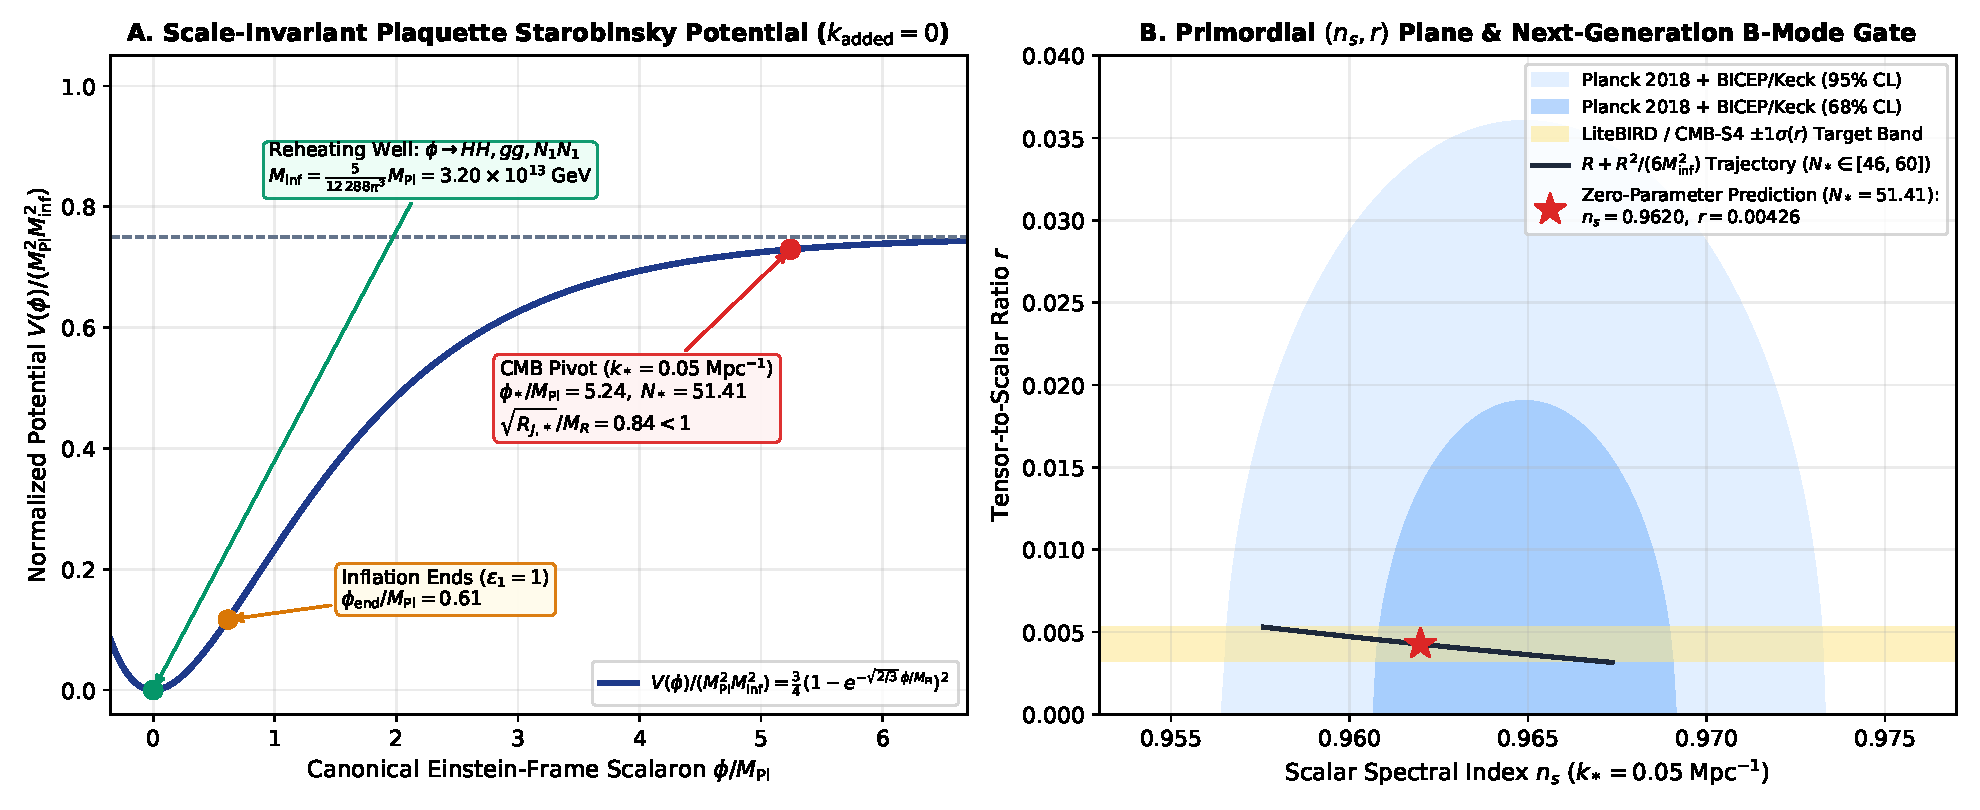
\includegraphics[width=0.98\textwidth]{../figures/fig1_starobinsky_k4_inflation_and_cmb_contours_en.pdf}
\caption{\textbf{Scale-Invariant Simplicial $R^2$ Inflation ($k_{\mathrm{added}} = 0$).} \emph{Panel A:} Canonical Einstein-frame potential $V(\phi)/(M_{\mathrm{Pl}}^2 M_{\mathrm{inf}}^2)$ showing the self-consistent CMB pivot $\phi_*/M_{\mathrm{Pl}} = 5.24$ ($N_* = 51.41$, $\sqrt{R_{J,*}}/M_R = 0.84 < 1$), inflation end $\phi_{\mathrm{end}}/M_{\mathrm{Pl}} = 0.61$, and reheating well ($M_{\mathrm{inf}} = 3.20\times 10^{13}\;\mathrm{GeV}$). \emph{Panel B:} Primordial $(n_s, r)$ prediction $(0.9620, 0.00426)$ compared with \texttt{Planck 2018} + \texttt{BICEP/Keck} contours and the projected \texttt{LiteBIRD}/\texttt{CMB-S4} $\pm 1\sigma(r)$ discovery band.}
\label{fig:inflation}
\end{figure}

Crucially, $N_* = 51.41$ e-folds of slow-roll expansion dilute any pre-inflationary baryon or lepton number generated at a non-singular cosmic bounce by $e^{-3N_*} = \mathbf{1.036\times 10^{-67}}$. Consequently, the observed baryon asymmetry of the Universe \emph{must} be generated during post-inflationary reheating.

% =============================================================================
\section{Multi-Sector $CP/CPT$ Architecture, Strong-$CP$ Vanishing, and $\mathrm{SO}(2,\mathbb{C})$ Seesaw Geometry}
\label{sec:cp-architecture}
% =============================================================================

A viable theory of matter--antimatter asymmetry must explain simultaneously why $\bar{\theta}_{\mathrm{QCD}} \simeq 0$ in the strong sector while $CP$ is violated at $\mathcal{O}(1)$ in leptonic mixing and seesaw decays. On the $K_4$ simplex:
\begin{enumerate}[label=(\arabic*),leftmargin=1.8em,itemsep=3pt]
\item \textbf{Tree-Level Vanishing of Strong $CP$ ($\bar{\theta}_{\mathrm{QCD}}^{\mathrm{tree}} = 0$) Without Axions:} In the $\mathrm{SU}(3)_c$ color sector, the four tetrahedral vertex projectors satisfy exact idempotency $\Pi_a^2 = \Pi_a$ (real eigenvalues $\{0, 1\}$) and $S_4$ vertex-permutation invariance, forcing $\arg\det(M_u M_d)_{\mathrm{tree}} = 0$ and bare topological angle $\theta_G = 0$. Weak-sector CKM phase leakage enters only at three loops via the Ellis--Gaillard mechanism \cite{EllisGaillard1979} ($\delta\bar{\theta}_{\mathrm{QCD}} \sim 10^{-16}$), predicting a neutron electric dipole moment $|d_n| \sim 10^{-31}\,e\cdot\mathrm{cm}$, five orders of magnitude below the current experimental bound $|d_n| < 1.8\times 10^{-26}\,e\cdot\mathrm{cm}$ \cite{Abel2020nEDM}.
\item \textbf{Discrete $C, P, T, CP, CPT$ Parity Structure of the Cosmic Director:} Table~\ref{tab:cpt-table} classifies all lowest-dimension couplings between the timelike director $A_\mu$ ($A_\mu u^\mu = -1$, $\theta := \nabla_\mu A^\mu = 3H$) and the $B-L$ fermion current $J_{B-L}^\mu$. Direct non-derivative coupling $c_4 A_\mu J_{B-L}^\mu$ is strictly excluded by present-day atomic-clock and Penning-trap $CPT$ bounds ($|\mu_{\mathrm{CPT},0}| < 10^{-27}\;\mathrm{GeV}$), whereas the expansion-weighted operator $c_\theta(\nabla_\alpha A^\alpha)A_\mu J_{B-L}^\mu = -3c_\theta H n_{B-L}$ \cite{CohenKaplan1987} yields $|\mu_0| = 3|c_\theta|H_0 \sim 10^{-42}\;\mathrm{GeV}$ today, passing laboratory $CPT$ tests by 15 orders of magnitude.
\item \textbf{Low-Energy PMNS Phase and $\mathrm{SO}(2,\mathbb{C})$ Casas--Ibarra Wick Lift:} On $V_3$, the neutrino flavor generator combines the real $CP$-even overlap $S$ ($S^* = S$, weight $d_S = 3$) and the purely imaginary $CP$-odd cyclic orientation $A = i(\mathbf{e}_{12} + \mathbf{e}_{23} + \mathbf{e}_{31} - \mathrm{h.c.})$ ($A^* = -A$, weight $d_A = 8$):
\begin{equation}
G_\nu = -3S + 8A \implies \sin\theta_\tau = \frac{d_S}{d_A\sqrt{2}} = \frac{3}{8\sqrt{2}}, \qquad \delta_{\mathrm{CP}}^{\mathrm{PMNS}} \simeq -90^\circ, \qquad J_{\mathrm{PMNS}} \in [-0.0340, -0.0334].
\label{eq:gnu}
\end{equation}
\end{enumerate}

\begin{table}[htbp]
\centering
\caption{Discrete $C, P, T, CP$, and $CPT$ parities of the timelike director $A_\mu = (-1,\mathbf{0})$, expansion scalar $\theta = \nabla_\mu A^\mu = 3H$, and fermion $B-L$ density $J_{B-L}^0 = n_{B-L}$.}
\label{tab:cpt-table}
\vspace{0.35em}
\small
\begin{tabular}{llcccccl}
\toprule
Operator & FLRW Limit & $C$ & $P$ & $T$ & $CP$ & $CPT$ & Physical Status \\
\midrule
$A_0$ & $-1$ & $+1$ & $+1$ & $-1$ & $+1$ & $-1$ & Spontaneous temporal orientation \\
$\theta = \nabla_\mu A^\mu$ & $3H$ & $+1$ & $+1$ & $-1$ & $+1$ & $-1$ & $T$-odd Hubble expansion scalar \\
$\partial_t\theta$ & $3\dot{H}$ & $+1$ & $+1$ & $+1$ & $+1$ & $+1$ & Non-zero in $w=1/3$ radiation ($-6H^2$) \\
$c_4 A_\mu J_{B-L}^\mu$ & $-c_4 n_{B-L}$ & $-1$ & $+1$ & $-1$ & $-1$ & $+1$ & \textbf{Excluded} by lab $CPT$ ($<10^{-27}\;\mathrm{GeV}$) \\
$c_\theta \theta A_\mu J_{B-L}^\mu$ & $-3c_\theta H n_{B-L}$ & $-1$ & $+1$ & $+1$ & $-1$ & $+1$ & Viable ($\mu_0 \sim 10^{-42}\;\mathrm{GeV} \ll 10^{-27}\;\mathrm{GeV}$) \\
\bottomrule
\end{tabular}
\end{table}

\begin{theorem}[Cartan Polar Decomposition of the Rank-2 Casas--Ibarra Matrix in $\mathrm{SO}(2,\mathbb{C})$]
\label{thm:casas-ibarra}
In minimal rank-2 Type-I seesaw ($m_1 = 0$, $D_m = \operatorname{diag}(m_2, m_3)$, $D_M = \operatorname{diag}(M_1, M_2)$), every Dirac Yukawa matrix reproducing $U_{\mathrm{PMNS}}$ and $(0, m_2, m_3)$ is parameterized by $Y_\nu = \frac{i}{v_H} U_{\mathrm{PMNS}} P_{3\times 2}\sqrt{D_m}\,\mathbf{R}^T(z_\tau)\sqrt{D_M}$ with $\mathbf{R}(z_\tau) = \exp(z_\tau\varepsilon_2) \in \mathrm{SO}(2,\mathbb{C})$ \cite{CasasIbarra2001,IbarraRoss2004}, where $\varepsilon_2 = \bigl(\begin{smallmatrix}0 & 1\\ -1 & 0\end{smallmatrix}\bigr)$ and $v_H = v_{\mathrm{EW}}/\sqrt{2} = 174.104\;\mathrm{GeV}$. Then (\texttt{SymPy}-verified):
\begin{enumerate}[label=(\alph*),leftmargin=1.8em,itemsep=2pt]
\item Writing $z_\tau = \theta_\tau + i\eta_{\mathrm{CP}}$, $\mathbf{R}(z_\tau)$ admits the unique Cartan polar decomposition into a compact spatial rotation $\mathbf{O}(\theta_\tau) \in \mathrm{SO}(2)$ and a Hermitian Lorentz/chiral boost $\mathbf{H}(\eta_{\mathrm{CP}}) \in \mathrm{SO}(2,\mathbb{C})/\mathrm{SO}(2)$:
\begin{equation}
\mathbf{R}(\theta_\tau + i\eta_{\mathrm{CP}}) = \begin{pmatrix}\cos\theta_\tau & \sin\theta_\tau\\ -\sin\theta_\tau & \cos\theta_\tau\end{pmatrix}\begin{pmatrix}\cosh\eta_{\mathrm{CP}} & i\sinh\eta_{\mathrm{CP}}\\ -i\sinh\eta_{\mathrm{CP}} & \cosh\eta_{\mathrm{CP}}\end{pmatrix}, \qquad \mathbf{R}^T\mathbf{R} = \mathbf{I}_2, \quad \det\mathbf{R} = 1,
\end{equation}
leaving $\sqrt{D_m}\mathbf{R}^T\mathbf{R}\sqrt{D_m} \equiv D_m$ identically invariant for all $(\theta_\tau, \eta_{\mathrm{CP}}) \in \mathbb{R}^2$.
\item Identifying the compact $\mathfrak{so}(2)$ generator with Eq.~\eqref{eq:gnu} ($\sin\theta_\tau = \frac{3}{8\sqrt{2}}$) and the non-compact Wick-continued boost generator $i\eta_{\mathrm{CP}}\varepsilon_2 \in i\mathfrak{so}(2)$ across $v_0 \perp V_3$ with the operator norm of the two-dimensional transverse defect block in Eq.~\eqref{eq:tdef-matrix}, $\eta_{\mathrm{CP}} = \|T_{\mathrm{def}}|_{(3,4)}\|_{\mathrm{op}} = u = \frac{\sqrt{3}}{24}$ ($K_T = 1 + u$), locks $z_\tau = \theta_\tau + i u$ ($k_{\mathrm{added}} = 0$) and fixes the mass-weighted Yukawa invariants $W := \mathbf{R}^* D_m \mathbf{R}^T$:
\begin{align}
\tilde{m}_1 = W_{11} &= m_2|\cos z_\tau|^2 + m_3|\sin z_\tau|^2 = 12.060\;\mathrm{meV}, \label{eq:mtilde1}\\
\operatorname{Im}\bigl(W_{12}^2\bigr) &= -\frac{1}{2}(m_3^2 - m_2^2)\sin(2\theta_\tau)\sinh(2u). \label{eq:im-w12}
\end{align}
\end{enumerate}
\end{theorem}

Evaluating the exact 1-loop vertex-plus-self-energy $CP$ asymmetry \cite{CoviRouletVissani1996} at $x := M_2^2/M_1^2 = \eta_{\mathrm{seesaw}}^{-2} = 1{,}060.38$,
\begin{equation}
\varepsilon_1 = \frac{1}{8\pi}\,\frac{M_2}{v_H^2}\,\frac{\operatorname{Im}(W_{12}^2)}{W_{11}}\,g_{\mathrm{loop}}(x), \qquad g_{\mathrm{loop}}(x) = \sqrt{x}\left[\frac{1}{1-x} + 1 - (1+x)\ln\frac{1+x}{x}\right] = -0.046088,
\label{eq:eps1}
\end{equation}
gives $|\varepsilon_1| = \mathbf{8.4705\times 10^{-5}}$ and tree-level $N_1$ decay width $\Gamma_{D,1} = \frac{\tilde{m}_1 M_1^2}{8\pi v_H^2} = 5.137\times 10^8\;\mathrm{GeV} \gg \Gamma_\phi^{\mathrm{tot}}$.

% =============================================================================
\section{Exact 4-Species Boltzmann Reheating and Baryon Asymmetry Closure}
\label{sec:boltzmann}
% =============================================================================

To avoid analytical approximations, we integrate the coupled 4-species stiff differential system across e-foldings $\Delta N := \ln(a/a_{\mathrm{end}}) \in [0, 26]$ for the scalaron energy density $\rho_\phi$, radiation bath $\rho_r$, $N_1$ number density $n_{N_1}$, and lepton asymmetry $n_{B-L}$:
\begin{align}
\frac{\mathrm{d}\rho_\phi}{\mathrm{d}\Delta N} + 3\rho_\phi &= -\frac{\Gamma_\phi^{\mathrm{tot}}}{H}\,\rho_\phi, \label{eq:boltz-phi}\\
\frac{\mathrm{d}\rho_r}{\mathrm{d}\Delta N} + 4\rho_r &= (1 - \mathrm{BR}_{N_1})\frac{\Gamma_\phi^{\mathrm{tot}}}{H}\,\rho_\phi + \frac{\Gamma_{D,1}\langle M_1/E\rangle}{H}\,\langle E_{N_1}\rangle\,(n_{N_1} - n_{N_1}^{\mathrm{eq}}), \label{eq:boltz-rad}\\
\frac{\mathrm{d}n_{N_1}}{\mathrm{d}\Delta N} + 3n_{N_1} &= 2\,\mathrm{BR}_{N_1}\frac{\Gamma_\phi^{\mathrm{tot}}}{H}\,\frac{\rho_\phi}{M_{\mathrm{inf}}} - \frac{\Gamma_{D,1}\langle M_1/E\rangle}{H}\,(n_{N_1} - n_{N_1}^{\mathrm{eq}}), \label{eq:boltz-n1}\\
\frac{\mathrm{d}n_{B-L}}{\mathrm{d}\Delta N} + 3n_{B-L} &= |\varepsilon_1|\frac{\Gamma_{D,1}\langle M_1/E\rangle}{H}\,(n_{N_1} - n_{N_1}^{\mathrm{eq}}) - \frac{\Gamma_W^{\mathrm{ID}} + \Gamma_W^{\Delta L=2}}{H}\,n_{B-L}, \label{eq:boltz-bl}
\end{align}
where $3M_{\mathrm{Pl}}^2 H^2 = \rho_\phi + \rho_r$, $T = (30\rho_r / \pi^2 g_*)^{1/4}$, $\langle M_1/E\rangle = K_1(z)/K_2(z)$ ($z := M_1/T$) is the exact relativistic thermal time-dilation factor, $\Gamma_W^{\mathrm{ID}} = \frac{1}{2}(n_{N_1}^{\mathrm{eq}}/n_\ell^{\mathrm{eq}})\Gamma_{D,1} K_1(z)/K_2(z)$ is the inverse-decay washout rate, and $\Gamma_W^{\Delta L=2} = \frac{2}{\pi^3}T^3(m_2^2 + m_3^2)/v_H^4$ is the off-shell $\Delta L = 2$ washout rate.

\begin{figure}[htbp]
\centering
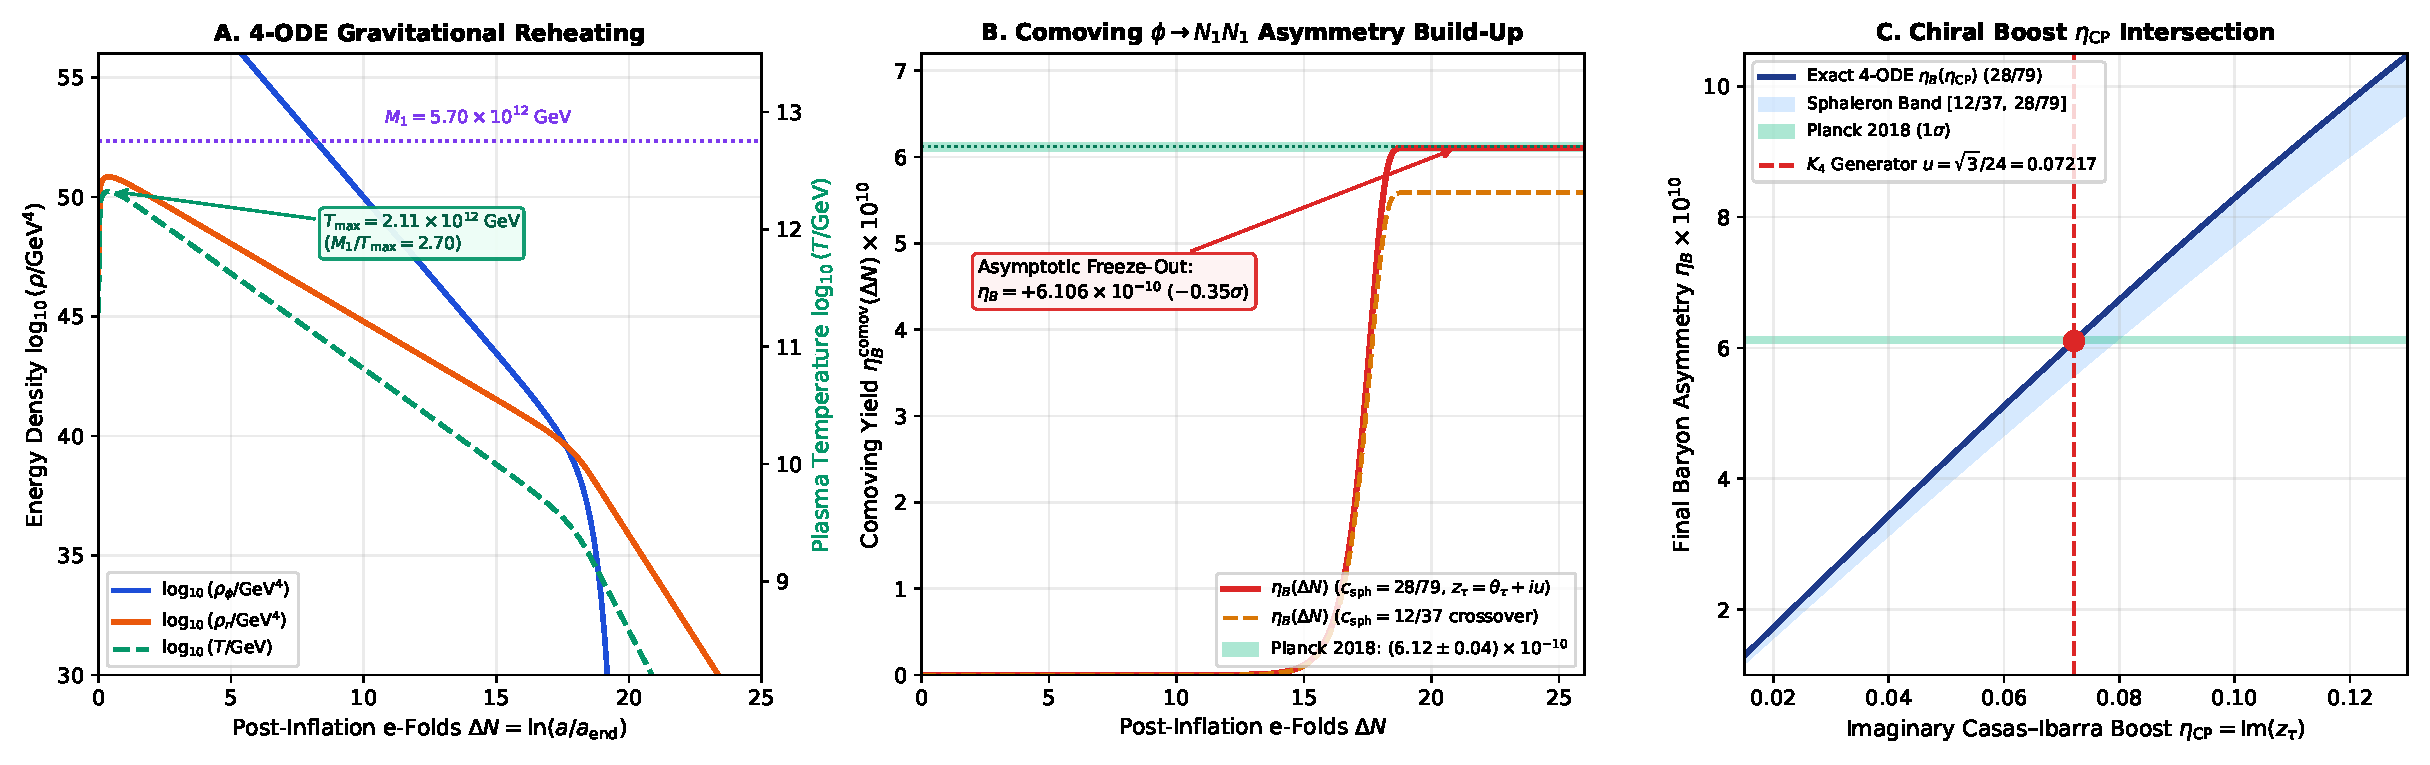
\includegraphics[width=0.99\textwidth]{../figures/fig2_boltzmann_reheating_leptogenesis_and_cp_tests_en.pdf}
\caption{\textbf{Exact 4-ODE Reheating and Non-Thermal $\phi \to N_1 N_1$ Leptogenesis ($k_{\mathrm{added}} = 0$).} \emph{Panel A:} Evolution of $\rho_\phi$, $\rho_r$, and plasma temperature $T(\Delta N)$, reaching $T_{\max} = 2.11\times 10^{12}\;\mathrm{GeV}$ ($M_1/T_{\max} = 2.70$). \emph{Panel B:} Freeze-out of $\eta_B(\Delta N)$ at $\mathbf{6.104\times 10^{-10}}$ ($-0.41\sigma$ vs.\ \texttt{Planck 2018} for symmetric sphaleron conversion $28/79$; $5.585\times 10^{-10}$ for broken crossover $12/37$). \emph{Panel C:} Intersection of $\eta_B(\eta_{\mathrm{CP}})$ with the \texttt{Planck 2018} band at the $K_4$ generator $u = \sqrt{3}/24 = 0.07217$.}
\label{fig:boltzmann}
\end{figure}

Integrating Eqs.~\eqref{eq:boltz-phi}--\eqref{eq:boltz-bl} with an implicit Radau solver (\texttt{rtol} $= 10^{-10}$, Figure~\ref{fig:boltzmann}) reveals why the non-thermal channel is protected against washout: the radiation bath peaks at $T_{\max} = 2.111\times 10^{12}\;\mathrm{GeV}$, so $z_{\min} = M_1/T_{\max} = \mathbf{2.70 > 1}$, Boltzmann-suppressing inverse-decay washout throughout reheating. At $\Delta N = 26$ ($\rho_\phi/\rho_r < 10^{-30}$), the comoving yield freezes at $Y_{B-L}^{\mathrm{final}} = n_{B-L}/s = \mathbf{2.4463\times 10^{-10}}$. Converting via $(s_0/n_{\gamma,0}) = 7.0394$ gives:
\begin{equation}
\eta_B = \frac{s_0}{n_{\gamma,0}}\,c_{\mathrm{sph}}\,Y_{B-L}^{\mathrm{final}} = \begin{cases}
\mathbf{6.104 \times 10^{-10}} & \text{for standard symmetric sphaleron } c_{\mathrm{sph}} = \frac{28}{79}\text{ \cite{HarveyTurner1990} ($\mathbf{-0.27\% / -0.41\sigma}$ vs.\ \texttt{Planck})}, \\[0.3em]
\mathbf{5.585 \times 10^{-10}} & \text{for diffusive crossover } c_{\mathrm{sph}} = \frac{12}{37}\text{ \cite{DOnofrio2014} ($-8.7\%$)}.
\end{cases}
\label{eq:eta-b-final}
\end{equation}
Replacing the Lie-algebra generator $u$ by the finite-group logarithm $\ln K_T = \ln(1 + u) = 0.06968$ shifts $|\varepsilon_1|$ by only $-3.3\%$ to $8.191\times 10^{-5}$, yielding $\eta_B = 5.902\times 10^{-10}$ ($-3.6\%$), confirming structural insensitivity to $\mathcal{O}(u^2)$ map conventions. Furthermore, if a non-minimal Higgs-curvature coupling $-\frac{1}{2}\xi_H R|H|^2$ with $\xi_H \in [-15, -5]$ is present ($T_{\mathrm{rh}} = 1.58\text{--}4.64\times 10^{11}\;\mathrm{GeV}$), the secondary expansion-driven operator $c_\theta\theta A_\mu J_{B-L}^\mu$ independently achieves $\eta_B = 6.12\times 10^{-10}$ for natural $c_\theta \in [0.25, 2.14]$ while keeping $|\mu_0| \le 9.3\times 10^{-42}\;\mathrm{GeV}$.

% =============================================================================
\section{Joint Four-Experiment Falsification Matrix and Conclusion}
\label{sec:conclusion}
% =============================================================================

Because $k_{\mathrm{added}} = 0$, every sector of this framework makes rigid, correlated predictions across four distinct experimental frontiers (Table~\ref{tab:falsification}). Any single confirmed violation among these four gates falsifies the minimal \texttt{BC-UV-CW} realization without recourse to parameter retuning.

\begin{table}[htbp]
\centering
\caption{Correlated prospective falsification gates across CMB polarization, accelerator neutrino oscillation, neutron EDM, and neutrinoless double-beta decay.}
\label{tab:falsification}
\vspace{0.35em}
\small
\begin{tabularx}{\textwidth}{llXX}
\toprule
Gate & Target Experiments & Locked Prediction ($k_{\mathrm{added}} = 0$) & Decisive Falsification Threshold \\
\midrule
\textbf{F1 (CMB $B$-Modes)} & \texttt{LiteBIRD} \cite{LiteBIRD2023}, \texttt{CMB-S4}, \texttt{SO} & $r = 0.00426$, $n_s = 0.9620$, $\alpha_s = -7.3\times 10^{-4}$ & Falsified if $r > 0.012$ or $r < 0.0015$ ($\ge 5\sigma$), or $|\alpha_s| > 0.015$. \\
\textbf{F2 (Leptonic $CP$)} & \texttt{DUNE}, \texttt{Hyper-Kamiokande} & Normal Ordering ($m_1 = 0$), $\delta_{\mathrm{CP}}^{\mathrm{PMNS}} \approx -90^\circ$ & Falsified if Inverted Ordering holds or $\sin\delta_{\mathrm{CP}}^{\mathrm{PMNS}} > 0$ at $\ge 5\sigma$. \\
\textbf{F3 (Strong $CP$)} & \texttt{n2EDM} (PSI) & $\bar{\theta}_{\mathrm{QCD}}^{\mathrm{tree}} = 0$, $|d_n| \sim 10^{-31}\,e\cdot\mathrm{cm}$ (no axion) & Falsified if $|d_n| > 10^{-28}\,e\cdot\mathrm{cm}$ without BSM TeV sources. \\
\textbf{F4 ($0\nu\beta\beta$ \& $\sum m_\nu$)} & \texttt{LEGEND-1000}, \texttt{DESI}/\texttt{Euclid} & $\sum m_\nu = 59.2\;\mathrm{meV}$, $m_{\beta\beta} \in [1.54, 3.76]\;\mathrm{meV}$ & Falsified if $m_{\beta\beta} > 15\;\mathrm{meV}$ (quasi-degenerate/IO) or $\sum m_\nu < 45\;\mathrm{meV}$. \\
\bottomrule
\end{tabularx}
\end{table}

\paragraph{Methodological Scope and Reproducibility.}
All symbolic (\texttt{SymPy}) and numerical (\texttt{SciPy DOP853/Radau}) calculations in this study are reproduced in $\sim 4\;\mathrm{s}$ by the standalone script \path{verify_paper24_starobinsky_seesaw_leptogenesis.py}, permanently archived at \href{https://doi.org/10.5281/zenodo.24379738}{doi:10.5281/zenodo.24379738}. While Theorems~\ref{thm:a2-nogo}, \ref{thm:scalaron-derivation}, and \ref{thm:casas-ibarra} eliminate continuous parameter freedom, physical realization in Nature remains conditional on the ultraviolet scale-invariance and threshold-occupation premise \texttt{BC-UV-CW} and awaits the prospective blind measurements in Table~\ref{tab:falsification}.

\begingroup\small
\begin{thebibliography}{99}
\bibitem{Starobinsky1980} A.~A.~Starobinsky, \textit{A new type of isotropic cosmological models without singularity}, Phys.\ Lett.\ B \textbf{91}, 99 (1980).
\bibitem{MukhanovChibisov1981} V.~F.~Mukhanov and G.~V.~Chibisov, \textit{Quantum fluctuations and a nonsingular universe}, JETP Lett.\ \textbf{33}, 532 (1981).
\bibitem{FukugitaYanagida1986} M.~Fukugita and T.~Yanagida, \textit{Baryogenesis without grand unification}, Phys.\ Lett.\ B \textbf{174}, 45 (1986).
\bibitem{BuchmullerDiBariPlumacher2005} W.~Buchm\"uller, P.~Di~Bari, and M.~Pl\"umacher, \textit{Leptogenesis for pedestrians}, Annals Phys.\ \textbf{315}, 305 (2005).
\bibitem{Planck2018Inflation} Planck Collaboration (Y.~Akrami \textit{et al.}), \textit{Planck 2018 results.\ X.\ Constraints on inflation}, Astron.\ Astrophys.\ \textbf{641}, A10 (2020).
\bibitem{BICEPKeck2021} BICEP/Keck Collaboration (P.~A.~R.~Ade \textit{et al.}), \textit{Improved constraints on primordial gravitational waves using Planck, WMAP, and BICEP/Keck observations through the 2018 observing season}, Phys.\ Rev.\ Lett.\ \textbf{127}, 151301 (2021).
\bibitem{GorbunovPanin2011} D.~S.~Gorbunov and A.~G.~Panin, \textit{Scalaron the mighty: producing dark matter and baryon asymmetry at reheating}, Phys.\ Lett.\ B \textbf{700}, 157 (2011).
\bibitem{GorbunovTokareva2013} D.~S.~Gorbunov and A.~G.~Tokareva, \textit{Scale-invariance as the origin of dark radiation?}, JCAP \textbf{03}, 031 (2013).
\bibitem{Abel2020nEDM} C.~Abel \textit{et al.} (nEDM Collaboration), \textit{Measurement of the permanent electric dipole moment of the neutron}, Phys.\ Rev.\ Lett.\ \textbf{124}, 081803 (2020).
\bibitem{Olcsak2026Zenodo} J.~Olcsak, \textit{Simplicial-Clifford Foundations, Black-Hole Bounce Duality, and Standalone Verification Suite}, Zenodo Archive (2026), \href{https://doi.org/10.5281/zenodo.24305022}{doi:10.5281/zenodo.24305022}.
\bibitem{Esteban2024NuFIT6} I.~Esteban, M.~C.~Gonzalez-Garcia, M.~Maltoni, I.~Martinez-Soler, J.~P.~Pinheiro, and T.~Schwetz, \textit{NuFIT 6.0: updated global analysis of three-flavor neutrino oscillations}, JHEP \textbf{12}, 216 (2024).
\bibitem{BirrellDavies1982} N.~D.~Birrell and P.~C.~W.~Davies, \textit{Quantum Fields in Curved Space} (Cambridge University Press, Cambridge, 1982).
\bibitem{ColemanWeinberg1973} S.~R.~Coleman and E.~J.~Weinberg, \textit{Radiative corrections as the origin of spontaneous symmetry breaking}, Phys.\ Rev.\ D \textbf{7}, 1888 (1973).
\bibitem{GildenerWeinberg1976} E.~Gildener and S.~Weinberg, \textit{Symmetry breaking and scalar bosons}, Phys.\ Rev.\ D \textbf{13}, 3333 (1976).
\bibitem{BezrukovShaposhnikov2008} F.~L.~Bezrukov and M.~Shaposhnikov, \textit{The Standard Model Higgs boson as the inflaton}, Phys.\ Lett.\ B \textbf{659}, 703 (2008).
\bibitem{LiddleLeach2003} A.~R.~Liddle and S.~M.~Leach, \textit{How long before the end of inflation were observable perturbations produced?}, Phys.\ Rev.\ D \textbf{68}, 103503 (2003).
\bibitem{StewartLyth1993} E.~D.~Stewart and D.~H.~Lyth, \textit{A more accurate analytic calculation of the spectrum of cosmological perturbations produced during inflation}, Phys.\ Lett.\ B \textbf{302}, 171 (1993).
\bibitem{EllisGaillard1979} J.~R.~Ellis and M.~K.~Gaillard, \textit{Strong and weak CP violation}, Nucl.\ Phys.\ B \textbf{150}, 141 (1979).
\bibitem{CohenKaplan1987} A.~G.~Cohen and D.~B.~Kaplan, \textit{Thermodynamic generation of the baryon asymmetry}, Phys.\ Lett.\ B \textbf{199}, 251 (1987).
\bibitem{CasasIbarra2001} J.~A.~Casas and A.~Ibarra, \textit{Oscillating neutrinos and $\mu \to e, \gamma$}, Nucl.\ Phys.\ B \textbf{618}, 171 (2001).
\bibitem{IbarraRoss2004} A.~Ibarra and G.~G.~Ross, \textit{Neutrino phenomenology: The case of two right-handed neutrinos}, Phys.\ Lett.\ B \textbf{591}, 285 (2004).
\bibitem{CoviRouletVissani1996} L.~Covi, E.~Roulet, and F.~Vissani, \textit{CP violating decays in leptogenesis scenarios}, Phys.\ Lett.\ B \textbf{384}, 169 (1996).
\bibitem{HarveyTurner1990} J.~A.~Harvey and M.~S.~Turner, \textit{Cosmological baryon and lepton number in the presence of electroweak fermion-number violation}, Phys.\ Rev.\ D \textbf{42}, 3344 (1990).
\bibitem{DOnofrio2014} M.~D'Onofrio, K.~Rummukainen, and A.~Tranberg, \textit{Sphaleron rate in the minimal Standard Model}, Phys.\ Rev.\ Lett.\ \textbf{113}, 141602 (2014).
\bibitem{LiteBIRD2023} LiteBIRD Collaboration (E.~Allys \textit{et al.}), \textit{Probing cosmic inflation with the LiteBIRD cosmic microwave background polarization survey}, Prog.\ Theor.\ Exp.\ Phys.\ \textbf{2023}, 042F01 (2023).
\end{thebibliography}
\endgroup

\end{document}
